%!TEX program = xelatex

\documentclass[11pt,titlepage]{report}
%!TEX root = main.tex

\usepackage[T1]{fontenc}
\usepackage{lmodern}
\usepackage[svgnames]{xcolor}
\usepackage{fontspec} % XeLaTeX required!
\usepackage{graphicx}
\usepackage{circuitikz}
\usepackage{tikz}
\usepackage{pifont}
\usepackage[some]{background}
\usepackage{xltxtra} 
\usepackage{setspace}
\usepackage[absolute]{textpos}
\usepackage[latin1]{inputenc}
\usepackage[english]{babel}
\usepackage{graphicx}
\usepackage{wrapfig}
\usepackage{fullpage}
\usepackage[margin=1in]{geometry}
\usepackage{float}
\usepackage{url}
\usepackage{multicol}
\usepackage{hyperref}
\usepackage{titlepic}
\usepackage{standalone}
\usepackage{siunitx}
\usepackage{booktabs}
\usepackage{amsmath}
\usepackage{unicode-math}
\usepackage{verbatim}
\usepackage{enumitem}
\usepackage{listings}
\usepackage{multirow}
\usepackage{pgfplots}
\pgfplotsset{compat=1.8}
\usepackage{caption} 
\usepackage[parfill]{parskip}
\usepackage{import}
\usepackage[backend=bibtexu,texencoding=utf8,bibencoding=utf8,style=ieee,sortlocale=en_GB,language=auto]{biblatex}
\usepackage[strict,autostyle]{csquotes}
\usepackage[final]{pdfpages}
\usepackage{subcaption}
\usepackage{ifplatform}
%\captionsetup[table]{skip=10pt}


% Fix for includepdf bug in Mac OS X
\newcommand{\insertpdfpath}[1]{
	\ifwindows
	\newcommand{\insertpdf}[2]{\includepdf[pages=##1]{##2}}
	\else
	\newcommand{\insertpdf}[2]{\includepdf[pages=##1]{#1/##2}}
	\fi
}

%set fonts
\setmainfont[Ligatures=TeX]{Myriad Pro}
\setmathfont{Asana Math}
\setmonofont{Lucida Console}

\usepackage{titlesec, color}
\renewcommand{\familydefault}{\sfdefault} %set font family
\renewcommand{\arraystretch}{1.2} %set table vertical spacing
\setlength\parindent{0pt} %no paragraph indent
\hypersetup{ %setup hyperlinks
    colorlinks,
    citecolor=black,
    filecolor=black,
    linkcolor=black,
    urlcolor=black
}

%redesign chapter headings
\definecolor{gray75}{gray}{0.75}
\newcommand{\chapternumber}{\thechapter}
\newcommand{\hsp}{\hspace{20pt}}
\titleformat{\chapter}[hang]{\Huge\bfseries}{\chapternumber\hsp\textcolor{gray75}{|}\hsp}{0pt}{\Huge\bfseries}

%Redefine appendix headers
\renewcommand{\appendixname}{Appendix}
\renewcommand{\appendixtocname}{Appendices}
\renewcommand{\appendixpagename}{Appendices}

%For code listings
\definecolor{black}{rgb}{0,0,0}
\definecolor{browntags}{rgb}{0.65,0.1,0.1}
\definecolor{bluestrings}{rgb}{0,0,1}
\definecolor{graycomments}{rgb}{0.4,0.4,0.4}
\definecolor{redkeywords}{rgb}{1,0,0}
\definecolor{bluekeywords}{rgb}{0.13,0.13,0.8}
\definecolor{greencomments}{rgb}{0,0.5,0}
\definecolor{redstrings}{rgb}{0.9,0,0}
\definecolor{purpleidentifiers}{rgb}{0.01,0,0.01}


\lstdefinestyle{csharp}{
language=[Sharp]C,
showspaces=false,
showtabs=false,
breaklines=true,
showstringspaces=false,
breakatwhitespace=true,
escapeinside={(*@}{@*)},
columns=fullflexible,
commentstyle=\color{greencomments},
keywordstyle=\color{bluekeywords}\bfseries,
stringstyle=\color{redstrings},
identifierstyle=\color{purpleidentifiers},
basicstyle=\ttfamily\small}

\lstdefinestyle{c}{
language=C,
showspaces=false,
showtabs=false,
breaklines=true,
showstringspaces=false,
breakatwhitespace=true,
escapeinside={(*@}{@*)},
columns=fullflexible,
commentstyle=\color{greencomments},
keywordstyle=\color{bluekeywords}\bfseries,
stringstyle=\color{redstrings},
identifierstyle=\color{purpleidentifiers},
}

\lstdefinestyle{matlab}{
language=Matlab,
showspaces=false,
showtabs=false,
breaklines=true,
showstringspaces=false,
breakatwhitespace=true,
escapeinside={(*@}{@*)},
columns=fullflexible,
commentstyle=\color{greencomments},
keywordstyle=\color{bluekeywords}\bfseries,
stringstyle=\color{redstrings},
identifierstyle=\color{purpleidentifiers}
}

\lstdefinestyle{vhdl}{
language=VHDL,
showspaces=false,
showtabs=false,
breaklines=true,
showstringspaces=false,
breakatwhitespace=true,
escapeinside={(*@}{@*)},
columns=fullflexible,
commentstyle=\color{greencomments},
keywordstyle=\color{bluekeywords}\bfseries,
stringstyle=\color{redstrings},
identifierstyle=\color{purpleidentifiers}
}

\lstdefinestyle{xaml}{
language=XML,
showspaces=false,
showtabs=false,
breaklines=true,
showstringspaces=false,
breakatwhitespace=true,
escapeinside={(*@}{@*)},
columns=fullflexible,
commentstyle=\color{greencomments},
keywordstyle=\color{redkeywords},
stringstyle=\color{bluestrings},
tagstyle=\color{browntags},
morestring=[b]",
  morecomment=[s]{<?}{?>},
  morekeywords={xmlns,version,typex:AsyncRecords,x:Arguments,x:Boolean,x:Byte,x:Char,x:Class,x:ClassAttributes,x:ClassModifier,x:Code,x:ConnectionId,x:Decimal,x:Double,x:FactoryMethod,x:FieldModifier,x:Int16,x:Int32,x:Int64,x:Key,x:Members,x:Name,x:Object,x:Property,x:Shared,x:Single,x:String,x:Subclass,x:SynchronousMode,x:TimeSpan,x:TypeArguments,x:Uid,x:Uri,x:XData,Grid.Column,Grid.ColumnSpan,Click,ClipToBounds,Content,DropDownOpened,FontSize,Foreground,Header,Height,HorizontalAlignment,HorizontalContentAlignment,IsCancel,IsDefault,IsEnabled,IsSelected,Margin,MinHeight,MinWidth,Padding,SnapsToDevicePixels,Target,TextWrapping,Title,VerticalAlignment,VerticalContentAlignment,Width,WindowStartupLocation,Binding,Mode,OneWay,xmlns:x}
}

\lstdefinestyle{matlab}{
language=Matlab,
showspaces=false,
showtabs=false,
breaklines=true,
showstringspaces=false,
breakatwhitespace=true,
escapeinside={(*@}{@*)},
columns=fullflexible,
commentstyle=\color{greencomments},
keywordstyle=\color{bluekeywords}\bfseries,
stringstyle=\color{purpleidentifiers},
identifierstyle=\color{purpleidentifiers}
}

%defaults
\lstset{
basicstyle=\ttfamily\small,
extendedchars=false,
numbers=left,
numberstyle=\ttfamily\tiny,
stepnumber=1,
tabsize=4,
numbersep=5pt
}
\addbibresource{../../library/bibliography.bib}

\begin{document}
\begin{appendices}
\renewcommand{\chapternumber}{\appendixname\space\thechapter} 

\chapter{Speed of sound}
\label{app:speed-of-sound}
Let us derive an expression for the speed of sound with herein the dependency on environment temperature and humidity. From the Newton-Laplace equation for the speed of sound in a medium

\begin{equation}
	c = \sqrt{\frac{K}{\rho}},
\end{equation}

where $K$ is a coefficient of stiffness (the bulk modulus) and $\rho$ the density of the medium in conjunction with the fact that for a gas holds that

\begin{equation}
	K = \gamma p,
\end{equation}

where $\gamma$ denotes the \emph{adiabatic index} of the gas and $p$ its pressure, yields the following expression:

\begin{equation} \label{eq:c1}
	c = \sqrt{\gamma \frac{p}{\rho}}.
\end{equation}

Assuming $\gamma$ and $p$ (being the \emph{total air pressure}) are known, we now need to find an expression for the density of the water-air mixture, $\rho$.
To accomplish this, we utilize the ideal gas law

\begin{equation}
	p V = n R T,
\end{equation}

with $V$ the gas volume, $n$ the number of molecules, $R$ the specific gas constant and $T$ the absolute temperature in Kelvin, together with the definition of density $\rho = n / V$ to obtain:

\begin{equation}
	\rho = \frac{p}{R T}.
\end{equation}

Now, since the density of a mixture can be written as the sum of the densities of the individual gases, we can write:

\begin{equation} \label{eq:rho1}
	\rho_{air} = \frac{p_a}{R_a T} + \frac{p_w}{R_w T},
\end{equation}

where $p_a$, $R_a$, $p_w$ and $R_w$ are the pressures and specific gas constants for dry air and water vapor respectively. However, since we like to express air humidity as a ratio between the current partial water pressure $e_w$ and the saturation water pressure $e^*_w$ at a given temperature:

\begin{equation}
	\phi = \frac{e_w}{e^*_w} \times 100\%,
\end{equation}

we can use the fact that $p_a = p_{tot} - p_w$ and $p_w = e_w$ to rewrite \ref{eq:rho1}:

\begin{equation} \label{eq:rho2}
	\rho_{air} = \frac{R_w(100 p_{tot} - \phi e^*_w) + 100 R_a \phi e^*_w}{10^4 R_a R_w T},
\end{equation}

which we can then substitute back into \ref{eq:c1} to obtain the required expression:

\begin{equation} \label{eq:c2}
	c = \sqrt{\gamma \frac{10^4 p_{tot} R_a R_w T}{100 R_w(100 p_{tot} - \phi e^*_w) + 100 R_a \phi e^*_w}}.
\end{equation}
\cite{sengpiel-sound-speed,uiuc-rel-humid,wikipedia-speed-of-sound}

\newcommand{\E}[1]{\operatorname{E}\left[#1\right]}
\newcommand{\Prob}[1]{\operatorname{P}\left[#1\right]}
\newcommand{\PSD}[1]{\operatorname{PSD}\left\{#1\right\}}
\let\F\Fold
\newcommand{\F}[1]{\mathcal{F}\left\{#1\right\}}
\newcommand{\Var}[1]{\operatorname{Var}\left[#1\right]}

\chapter{Signaling analysis}
\label{app:sig-an}


\section{Power analysis}
\subsection{PSD of an ASK signal}
Let us investigate the PSD of an ASK signal $s(t)$ given by
\begin{equation*}
	s(t) = A_c (1+\mu m_1(t)) \cos{(\omega_c t)}
\end{equation*}
where we assume that $m_1(t)$ is a polar NRZ line code. The autocorrelation function is given by
\begin{align*}
	R_s(\tau) &=\E{A_c (1+\mu m_1(t)) \cos{(\omega_c t)} A_c (1+\mu m_1(t+\tau)) \cos{(\omega_c (t+\tau))}} \\
	&=\E{A_c \cos{(\omega_c t)} A_c \cos{(\omega_c (t+\tau))} }\left( 1 + \mu^2 \E{m_1(t)} \E{m_1(t+\tau)}+ \mu^2 \E{m_1(t) m_1(t+\tau)}\right) \\
	&=R_c(\tau) + \mu^2 R_c(\tau) R_m(\tau).
\end{align*}
Fourier transforming $R_s(\tau)$ yields
\begin{align}
	\PSD{s(t)}(f) &= \F{R_s(\tau)} \nonumber \\
	&= \mu^2 \PSD{c(t)}(f) \ast \PSD{m_1(t)}(f) + \PSD{c(t)}(f) \nonumber \\
	&= \frac{A_c^2}{2} \delta(f-f_c) \ast \mu^2 \PSD{m_1(t)}(f) + \frac{A_c^2}{2} \delta(f-f_0) \nonumber \\
	&= \frac{A_c^2}{2} \left( \mu^2 \PSD{m_1(t)}(f-f_c) + \delta(f-f_c) \right). \label{eq:psd-ask}
\end{align}
\subsection{PSD of an FSK signal}
Let us now consider an FSK signal $s(t)=s_1(t)+s_2(t)$ where
\begin{align*}
	s_1(t) &= A_c m_2(t) \cos{(\omega_{c_1} t)} \text{ and } \\
	s_2(t) &= A_c (1-m_2(t)) \cos{(\omega_{c_2} t)}
\end{align*}
and we assume that $m_2(t)$ is a unipolar NRZ line code. Calculating the autocorrelation function of $s_1(t)$ yields
\begin{align*}
	R_{s_1}(\tau) &= \E{A_c m_2(t) \cos{(\omega_{c_1} t)} A_c m_2(t+\tau) \cos{(\omega_{c_1} (t+\tau))}} \\
	&= R_{c_1}(\tau) R_{m}(\tau).
\end{align*}
When we assume both bits have equal probability then
\begin{align*}
	\E{m_2(t)} = \frac{1}{2} \cdot 1 + \frac{1}{2} \cdot 0 = \frac{1}{2}.
\end{align*}
Calculating the autocorrelation function of $s_2(t)$ yields
\begin{align*}
	R_{s_2}(\tau) &= \E{A_c (1-m_2(t)) \cos{(\omega_{c_2} t)} A_c (1-m_2(t+\tau)) \cos{(\omega_{c_2} (t+\tau))}} \\
	&= \E{A_c\cos{(\omega_{c_2} t)} A_c \cos{(\omega_{c_2} (t+\tau))}}\left( 1 - \E{m_2(t)} - \E{m_2(t+\tau)} + \E{m_2(t)m_2(t+\tau)} \right) \\
	&= \E{A_c\cos{(\omega_{c_2} t)} A_c \cos{(\omega_{c_2} (t+\tau))}} \E{m_2(t)m_2(t+\tau)} \\
	&= R_{c_2}(\tau) R_{m}(\tau).
\end{align*}
Note that $s_1(t)$ and $s_2(t)$ are orthogonal.
\begin{align*}
	R_{s_1,s_2}(\tau)&=\E{A_c m_2(t) \cos{(\omega_{c_1} t)} A_c (1-m_2(t)) \cos{(\omega_{c_2} (t+\tau))}} \\
	&= \E{\cos{(\omega_{c_1} t)}\cos{(\omega_{c_2} (t+\tau))}} \E{A_c^2 m_2(t) (1-m_2(t))} = 0
\end{align*}
We can then calculate the autocorrelation function of $s(t)$.
\begin{align*}
	R_s(\tau)&=\E{(s_1(t)+s_2(t))(s_1(t+\tau)+s_2(t+\tau))} \\
	&=R_{s_1}(\tau)+R_{s_2}(\tau)
\end{align*}
Fourier transforming yields
\begin{align}
	\PSD{s_1(t)+s_2(t)} &= \F{R_{s_1}(\tau)}(f) + \F{R_{s_2}(\tau)}(f) \nonumber \\
	&= \PSD{s_1(t)}(f) + \PSD{s_2(t)}(f) \nonumber \\
	&= \frac{A_c^2}{2} \delta(f-f_{c_1}) \ast \PSD{m_2(t)}(f) + \frac{A_c^2}{2} \delta(f-f_{c_2}) \ast \PSD{m_2(t)}(f) \nonumber \\
	&= \frac{A_c^2}{2}\left( \PSD{m_2(t)}(f-f_{c_1}) + \PSD{m_2(t)}(f-f_{c_2}) \right). \label{eq:psd-fsk}
\end{align}
\subsection{Signal power}
We can now calculate the signal power of the evaluated ASK signal and FSK signal.
\begin{align*}
	\E{s_{\text{ASK}}^2(t)} &= \int_{-\infty}^{\infty} \PSD{s_{\text{ASK}}^2(t)}(f) df \\
	&= \frac{A_c^2}{2} \int_{-\infty}^{\infty}\left( \mu^2 \PSD{m_1(t)}(f-f_c) + \delta(f-f_c) \right) df \\
	&= \mu^2 \frac{A_c^2}{2}\E{m_1^2(t)} + \frac{A_c^2}{2}.
\end{align*}
\begin{align*}
	\E{s_{\text{FSK}}^2(t)} &= \int_{-\infty}^{\infty} s_{\text{FSK}}^2(t) df \\
	&= \frac{A_c^2}{2} \int_{-\infty}^{\infty} \left( \PSD{m_2(t)}(f-f_{c_1}) + \PSD{m_2(t)}(f-f_{c_2})\right) df \\
	&= A_c^2 \E{m_2^2(t)}
\end{align*}
\subsection{Spectral efficiency}
The spectral efficiencies of both signals are given by
\begin{align*}
	\eta_{\text{ASK}} &= \frac{\mu^2 \frac{A_c^2}{2}\E{m_1^2(t)}}{\mu^2 \frac{A_c^2}{2}\E{m_1^2(t)} + \frac{A_c^2}{2}} = \frac{\mu^2\E{m_1^2(t)}}{\mu^2\E{m_1^2(t)} + 1} \text{ and } \\
	\eta_{\text{FSK}} &= \frac{A_c^2 \E{m_2^2(t)}}{A_c^2 \E{m_2^2(t)}} = 1.
\end{align*}
\subsection{Signal quality comparison}
Using Equation \ref{eq:psd-ask} and \ref{eq:psd-fsk} and the fact that the bandwidth of both line codes $m_1(t)$ and $m_2(t)$ is equal to the data rate $R$, we can conclude that the transmission bandwidths of $s_{\text{ASK}}(t)$ and $s_{\text{FSK}}(t)$ are given by
\begin{align*}
	B_{\text{ASK}} &= 2R \text{ and } \\
	B_{\text{FSK}} &= 2(R + |f_{c_1} - f_{c_2}|) = 2(R + \Delta f).
\end{align*}
If we assume AWGN with a one-sided PSD of $N_0$, then the signal-to-noise ratio's are given by
\begin{align*}
	\left(\frac{S}{N}\right)_{\text{ASK}} &= \eta_{\text{ASK}} \frac{\mu^2 \frac{A_c^2}{2}\E{m_1^2(t)} + \frac{A_c^2}{2}}{2RN_0}, \\
	\left(\frac{S}{N}\right)_{\text{FSK}} &= \eta_{\text{FSK}} \frac{A_c^2 \E{m_2^2(t)} + \frac{A_c^2}{2}}{2(R+\Delta f)N_0}.
\end{align*}
If we assume equal probability of the transmitted bits, then the signal powers are easy to calculate.
\begin{align*}
	\E{m_1^2(t)} &= \frac{1}{2} \cdot 1^2 + \frac{1}{2} \cdot (-1)^2=1, \\
	\E{m_2^2(t)} &= \frac{1}{2} \cdot 1^2 + \frac{1}{2} \cdot 0^2=\frac{1}{2}.
\end{align*}
Substituting these results in the expressions for the signal-to-noise ratio's yields
\begin{align*}
	\left(\frac{S}{N}\right)_{\text{ASK}} &= \frac{\mu^2}{\mu^2+1} \frac{A_c^2 (\mu^2+1)}{4RN_0} = \frac{\mu^2 A_c^2}{4RN_0}, \\
	\left(\frac{S}{N}\right)_{\text{FSK}} &= \frac{A_c^2}{2(R+\Delta f)N_0}.
\end{align*}
We can now compare the obtained signal-to-noise ratio's.
\begin{align*}
	\frac{(S/N)_{\text{FSK}}}{(S/N)_{\text{ASK}}}=\frac{A_c^2}{2(R+\Delta f)N_0} \frac{4RN_0}{\mu^2 A_c^2}=\frac{R}{R+\Delta f}\frac{2}{\mu^2}
\end{align*}
We conclude that from a signal's power perspective for high bit rates ($R \gg \Delta f$) using FSK is advantageous.
\subsection{Spectral behaviour analysis}
We can determine a lot of properties of the PSD's of an ASK and FSK signal by inspecting Equations \ref{eq:psd-ask} and \ref{eq:psd-fsk}.

The spectrum of an ASK signal contains a delta pulse at the carrier frequency. The spectrum of the modulation signal is centered around this carrier frequency. The amplitude of the PSD is proportional to $\mu^2$. If we increase the bit rate, then the transmission bandwidth increases as the bandwidth of the modulation signal increases. Also, the amplitude of the spectrum will decrease by increasing the bit rate.

The spectrum of an FSK signal contains delta pulses at the two used frequencies. The spectrum of the modulation signal is centered around both of these frequencies. These delta pulses originate from the modulation signal, as they contain DC components. The PSD is in a same manner related to the bit rate as the PSD of an ASK signal.

\section{Noise analysis}
\subsection{Demodulation of ASK}
To demodulate an ASK signal, the stochastic variable $X=\widetilde{s}(t) A_c \cos{(\omega_c t + \phi)}$ is evaluated. Here $\widetilde{s}(t)=s(t)+n(t)$ denotes the received signal $s(t)$ with AWGN $n(t)$. The expectation value of $X$ is given by
\begin{align*}
	\E{X}&=\E{(s(t)+n(t)) A_c \cos{(\omega_c t + \phi)}} \\
	&=\E{\left(A_c (1+\mu m_1(t)) \cos{(\omega_c t)} + n(t)\right) A_c \cos{(\omega_c t + \phi)}} \\
	&= \E{(1+\mu m_1(t)) A_c^2 \frac{\cos{(\phi)} + \cos{(2 \omega_c t + \phi)}}{2}} + \E{n(t) A_c \cos{(\omega_c t + \phi)}} \\
	&= \frac{\cos{(\phi)} A_c^2}{2} \E{1+\mu m_1(t)} \\
	&= \frac{\cos{(\phi)} A_c^2}{2} \left( 1 + \mu \E{m_1(t)} \right)
\end{align*}
To decide the bit value of the received signal at time $t$, we compare $X$ to the so-called decision threshold $T$. If $X>T$, then a `1' is received, and if $X<T$, then a `0' is received. If we want this decision to be unbiased, then $X-T$ should be proportional to the expectation value of $m_1(t)$, which represents the actual bit sent.
\begin{align*}
	X - T &\sim \E{m_1(t)} \\
    \frac{\cos{(\phi)} A_c^2}{2} - T+ \frac{\cos{(\phi)} A_c^2}{2}  \mu \E{m_1(t)} &\sim \E{m_1(t)} \\
    T &= \frac{\cos{(\phi)} A_c^2}{2}
\end{align*}
To explore the effect of AWGN, we evaluate $\Var{X}=\E{X^2}-\E{X}^2$. 
\begin{align*}
	\E{X^2}&=\E{(s(t)+n(t))^2 A_c^2 \cos^2{(\omega_c t + \phi)}} \\
	&=\E{\left(s^2(t)+2n(t)s(t)+n^2(t)\right) A_c^2 \frac{1}{2} \left( 1+ \cos{(2\omega_c t + 2\phi)}\right)} \\
	&=\frac{A_c^2}{2}\E{s^2(t) + n^2(t)} \\
	&=\alpha + \frac{A_c^2}{2} \E{n^2(t)}
\end{align*}
Now, the variance is given by
\begin{align*}
	\Var{X} &= \E{X^2} - \E{X}^2 \\
	&= \alpha + \frac{A_c^2}{2} \E{n^2(t)} - \beta \\
	&= \alpha + \frac{A_c^2}{2} \Var{n(t)} - \beta
\end{align*}
We see that when the variance of the noise increases, the variance of $X$ increases and we consequently expect the bit error probability to increase. This result could also easily be explained by the fact that the signal-to-noise ratio decreases when $\Var{n^2(t)}$ increases.

\subsection{Demodulation of FSK}
We have shown that an FSK signal is a superposition of two signals with different frequencies. These signals are separated and evaluated in a same manner as an ASK signal. However, the information is now stored in the existence of a certain frequency instead of the amplitude of the received signal. As only the existence of a certain frequency has to be determined, the decision threshold can be set in a way that is less sensitive to noise than for an ASK signal.

\chapter{Relevant measurement results}
\label{app:res}

Table~\ref{tab:app-th} shows the measurement results in determining the optimal decision threshold for an ASK signal with carrier frequency \SI{1000}{Hz}, bit rate of \num{20} bits/s and modulation index of \num{1}.

\begin{table}[H]
	\centering
	\caption{Measurement results in determining the optimal decision threshold}
	\label{tab:app-th}
	\begin{tabular}{c c c}
		\hline\hline
		Noise STD & Decision threshold & BER \\
		\hline
		\num{0.05} & \num{0} & \num{0.55} \\ \hline
		\num{0.05} & \num{0.1} & \num{0.11} \\ \hline
		\num{0.05} & \num{0.2} & \num{0.00} \\ \hline
		\num{0.05} & \num{0.3} & \num{0.02} \\ \hline
		\num{0.05} & \num{0.4} & \num{0.05} \\ \hline
		\num{0.05} & \num{0.5} & \num{0.17} \\ \hline
		\num{0.05} & \num{0.6} & \num{0.29} \\ \hline
		\num{0.05} & \num{0.7} & \num{0.23} \\ \hline
		\hline
	\end{tabular}
\end{table}

Table~\ref{tab:app-noise} shows the measurement results of the BER for different noise standard deviations for an ASK signal with carrier frequency \SI{1000}{Hz}, bit rate of \num{20} bits/s, modulation index of \num{1} and decision threshold on \num{0.2}.

\begin{table}[H]
	\centering
	\caption{Measurement results in determining the optimal decision threshold}
	\label{tab:app-noise}
	\begin{tabular}{c c c}
		\hline\hline
		Noise STD & Decision threshold & BER \\
		\hline
		\num{0.1} & \num{0.2} & \num{0.11} \\ \hline
		\num{0.2} & \num{0.2} & \num{0.29} \\ \hline
		\num{0.3} & \num{0.2} & \num{0.26} \\ \hline
		\num{0.4} & \num{0.2} & \num{0.38} \\ \hline
		\num{0.5} & \num{0.2} & \num{0.32} \\ \hline
		\num{0.6} & \num{0.2} & \num{0.37} \\ \hline
		\num{0.7} & \num{0.2} & \num{0.38} \\ \hline
		\num{0.8} & \num{0.2} & \num{0.48} \\ \hline
		\hline
	\end{tabular}
\end{table}

Figure~\ref{fig:app-ask-br} shows the effect of altering the bit rate on the PSD of an ASK signal. The settings shown in Table \ref{tab:app-ask-br-settings} were used.

\begin{figure}[H]
	\begin{center}
		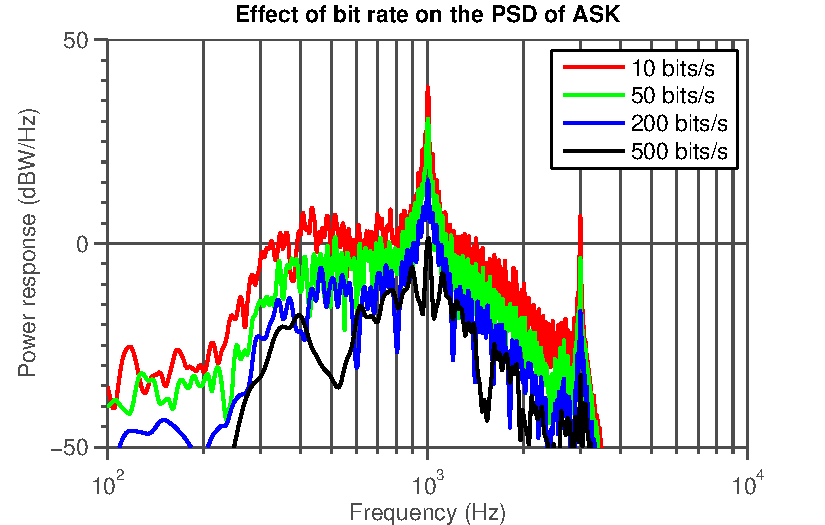
\includegraphics[width=0.8\linewidth]{resource/ask-br.pdf}
	\end{center}
	\caption{Effect of bit rate on the PSD of ASK}
	\label{fig:app-ask-br}
\end{figure}

\begin{table}[H]
	\centering
	\caption{Settings used when measuring the effect of altering the bit rate on the PSD of an ASK signal}
	\label{tab:app-ask-br-settings}
	\begin{tabular}{c c}
		\hline\hline
		Setting & Value \\
		\hline
		Modulation & ASK \\
		Modulation index & \num{1} \\
		Distance between source and receiver & \SI{10}{cm} \\
		Carrier frequency & \SI{1}{kHz} \\
		Decision threshold & \num{1} \\
		\hline
	\end{tabular}
\end{table}

Figure \ref{fig:app-fsk-peaks} shows the peaks we observed. The settings used are shown in Table \ref{tab:app-fsk-peaks-settings}.

\begin{figure}[H]
	\begin{center}
		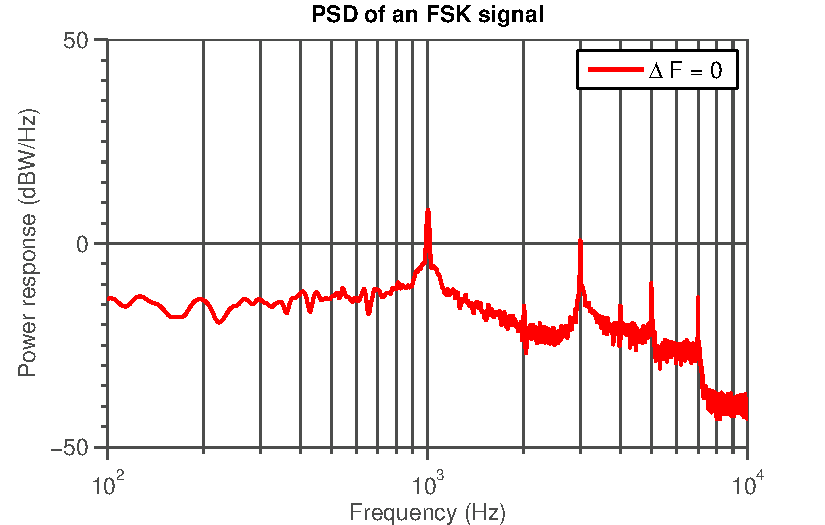
\includegraphics[width=0.8\linewidth]{resource/fsk-mod-1st.pdf}
	\end{center}
	\caption{Peaks we observed}
	\label{fig:app-fsk-peaks}
\end{figure}

\begin{table}[H]
	\centering
	\caption{Settings used when we encountered the peaks}
	\label{tab:app-fsk-peaks-settings}
	\begin{tabular}{c c}
		\hline\hline
		Setting & Value \\
		\hline
		Modulation & FSK \\
		Bit rate & \num{200} bits/s \\
		Distance between source and receiver & \SI{20}{cm} \\
		Carrier frequency & \SI{1}{kHz} \\
		Decision threshold & \num{1} \\
		\hline
	\end{tabular}
\end{table}

Figure~\ref{fig:app-ber} shows the best achieved bit error rates for a maximal bit rate with no ECC. The settings used are shown in Table~\ref{tab:app-ber}.

\begin{figure}[H]
	\begin{center}
		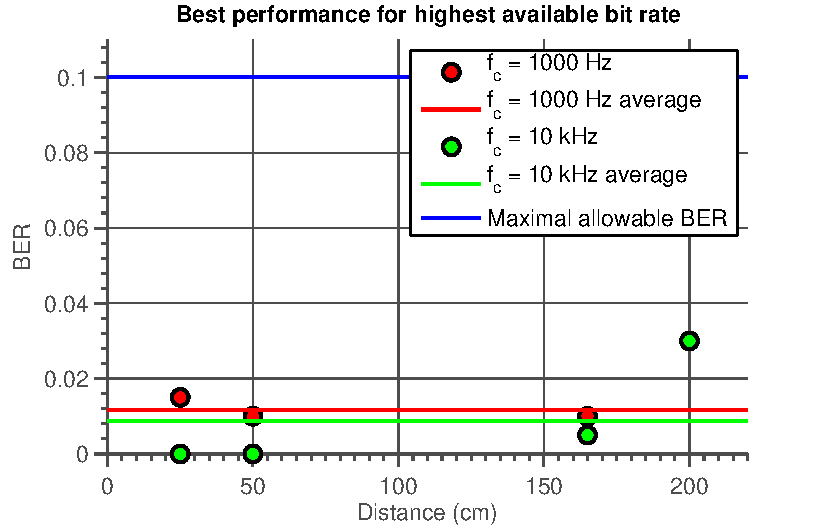
\includegraphics[width=0.8\linewidth]{resource/task-5.pdf}
	\end{center}
	\caption{Achieved bit error rates}
	\label{fig:app-ber}
\end{figure}

\begin{table}[H]
	\centering
	\caption{Settings used when determining the best achievable BER for a maximal information rate}
	\label{tab:app-ber}
	\begin{tabular}{c c}
		\hline\hline
		Setting & Value \\
		\hline
		Modulation & FSK \\
		$\Delta F$ & \SI{1}{kHz} \\
		Decision threshold & \num{0.6} \\
		\hline
	\end{tabular}
\end{table}

\end{appendices}
\end{document}